\chapter{Ондуляторное излучение}
В этой части мы дадим вывод излучения релятивистского электрона в $r\omega$-пространстве, движущегося в синусоидальном магнитном поле. Вывод замечателен тем, что даёт результаты из первых принципов --- уравнений Максвелла, а точность используемых приближений можно наглядно проследить по ходу изложения. В выкладках мы следовали подходу разработанному в серии работ \cite{geloni2005paraxial}, \cite{geloni2007fourier}, \cite{geloni2015brightness }, \cite{geloni2006fourier}. В заключении главы, будет дан обзор на подход, который используется в симуляционном коде SRW \cite{chubar1998proceedings}, а также даны краткие описания других симуляционных кодов, которые активно используются в научном сообществе для расчёта синхротронного излечения. 
\section{Излучение релятивистского электрона в синусоидальном магнитном поле}
\subsection{Уравнение движения электрона в ондуляторе}
Выведем спектр излучения ондулятора. Вывод начнём с уравнения движение релятивистского электрона в магнитном поле.

\begin{equation}
	\vec{F} = e[\vec{v} \times \vec{B}],
\end{equation} 
где $e$ --- заряд электрона, а $\vec{v}$ и $\vec{B}$ --- скорость частицы и магнитное поле, соответственно. Уравнение можно переписать в виде:

\begin{equation}
	\label{eq:NewTown}
	\cfrac{d\vec{p}}{dt} = \cfrac{e}{\gamma m_e}[\vec{v} \times \vec{B}],
\end{equation}
где $\gamma$ --- лоренц фактор, появившийся из релятивистского импульса. Отложим ось $z$ вдоль направления релятивистского движения электрона и будем считать, магнитное поле в ондуляторе $B_0\cos(k_w z)$ направлено вдоль оси $y$, где $k_w$ связана с периодом ондулятора следующим образом $k_w = 2\pi/\lambda_w$. После этого уравнение~\ref{eq:NewTown} можно переписать в виде:

\begin{equation}
	\label{eq:eq_of_motion}
	\begin{cases}
		\cfrac{d^2 x}{dt^2} = - \cfrac{e B_0}{\gamma m_e}\cfrac{dz}{dt} \cos(k_w z)\\
		\cfrac{d^2 z}{dt^2} = \cfrac{e B_0}{\gamma m_e}\cfrac{dx}{dt} \cos(k_w z)
	\end{cases} 
\end{equation}
далее, один раз интегрируя первое уравнение системы с заменой $dz = \beta cdt$, где $\beta = \|\vec{v}\| /c$, можно получить: 

\begin{equation}
 	\label{eq:dx/dt}
	\cfrac{dx}{dt} = - \cfrac{eB_0}{\gamma m_ek_w} \sin(k_w z)
\end{equation}
Введём коэффициент ондуляторности --- $K = \cfrac{eB_0 \lambda_u}{2 \pi m_e c}$, который показывает угол отклонения траектории электрона от оси $z$. 

Подставляя получившийся результат~\ref{eq:dx/dt} во второе уравнение системы~\ref{eq:eq_of_motion} и интегрируя с пределами от $0$ до некоторого $z_0$, получим систему:

\begin{equation}
	\begin{cases}
	\label{eq:eq_of_motion_velocity}
		\cfrac{dx}{dt} = - \cfrac{Kc}{\gamma} \sin(k_w z)\\
		\cfrac{dz}{dt} = \beta c - \cfrac{K^2 c}{2 \gamma^2 \beta}\sin^2(k_w z)
	\end{cases} 
\end{equation}
Чтобы получить уравнение на траекторию частицы, ещё раз проинтегрируем оба уравнения и получим:

\begin{equation}
	\begin{cases}
	\label{eq:eq_of_motion_trej}
		x = \cfrac{Kc}{\gamma k_w \beta} \cos(k_w\overline{\beta}ct)\\
		z = \overline{\beta}ct + \cfrac{K^2}{8 \beta^2 \gamma^2 k_w}\sin(2k_w\overline{\beta}ct) 
	\end{cases} 
\end{equation}
Здесь мы ввели обозначение $\overline{\beta}$, которое определяется как $\overline{\beta}c = \beta c\bigg(1 - \cfrac{K^2}{4 \beta^2 \gamma^2}\bigg)$. Полученные решения мы будем использовать при интегрировании уравнений Максвелла.
%Из~\ref{eq:eq_of_motion_velocity} видно, что продольная скорость испытывает о осцилляции с удвоенной частотой...
\subsection{Решение уравнений Максвелла в прааксиальном приближении}
Вывод спектра излучения будем проводить в $r\omega$-пространстве. Начнём с уравнений Максвелла в вакууме:
\begin{equation}
	\begin{cases}
		\nabla \cdot \vec{E} = 4\pi \rho\\
		\nabla \cdot \vec{B} = 0\\
		[\nabla \times \vec{E}] = -\cfrac{1}{c} \cfrac{\partial\vec{B}}{\partial t}\\
		[\nabla \times \vec{B}] = \cfrac{4\pi}{c} \vec{j} + \cfrac{1}{c} \cfrac{\partial\vec{E}}{\partial t}
	\end{cases} 
\end{equation}
Из уравнений тривиально можно получить неоднородное волновое уравнение: 
\begin{equation}
	\label{eq:inhomo_wave_eq_xt}
	c^2 \nabla^2 \vec{E} - \pdv[2]{\vec{E}}{t} = 4\pi c^2 \nabla \rho + 4\pi \pdv{\vec{j}}{t}
\end{equation}
Это же уравнение перепишем в $r\omega$-пространстве, определив преобразование Фурье следующим образом:
\begin{equation}
	\label{eq:Fourier_wt}
	\begin{array}{lcl}
		\vec{\widetilde{E}}(r, \omega) = \displaystyle\int\limits_{-\infty}^{\infty} dt \vec{E}(r, t)\exp[i\omega t]\\
		\\
		\vec{E}(r, \omega) = \cfrac{1}{2\pi}\displaystyle\int\limits_{-\infty}^{\infty} d\omega \vec{\widetilde{E}}(r, t)\exp[-i\omega t]
	\end{array}
\end{equation}
Применив к уравнению~\ref{eq:inhomo_wave_eq_xt}, получим:
\begin{equation}
	\label{eq:inhomo_wave_eq_xw}
	\omega^2 \vec{\widetilde{E}} + c^2 \nabla^2 \vec{\widetilde{E}} = 4\pi c^2 \nabla  \widetilde{\rho} - 4i\pi\omega\vec{\widetilde{j}}
\end{equation}
Перепишем это уравнение в приближении медленно меняющейся амплитуды в сравнение с частотой осцилляций, что есть $\vec{\widetilde{E}} =  \vec{\overline{E}}\exp[i\omega z/c]$, в приближении $\cfrac{\partial |\vec{E}|}{\partial z} \ll \cfrac{\omega}{c}|\vec{E}|$. Где временная зависимость разложена до нулевого порядка малости, исходя из уравнения~\ref{eq:eq_of_motion_trej} получим:
\begin{equation}
	\label{eq:wave_slow_vary}
	c^2\bigg(\nabla^2 \vec{\widetilde{E}} + \cfrac{2i\omega}{c}\pdv{\vec{\widetilde{E}}}{z}\bigg)\exp[i\omega z/c] = 4\pi c^2 \nabla  \widetilde{\rho} - 4i\pi\omega\vec{\widetilde{j}}
\end{equation}
Для электрона движущегося в вакууме ток и плотность заряда выражается через дельта-функцию Дирака:

\begin{equation}
	\begin{array}{lcl}
		\rho(r,t) = -e\delta(\vec{r}- \vec{r'}(t)) = -\cfrac{e}{v_z(z)}\delta(\vec{r}_{\bot}- \vec{r'}_{\bot}(z))\delta(\cfrac{s(z)}{v} - t)\\
		\vec{j}(r,t) = \vec{v}\rho(r,t)	
	\end{array}
\end{equation} 
В $r\omega$-пространстве: 
\begin{equation}
	\begin{array}{lcl}
		\widetilde{\rho}(r,\omega) = -\cfrac{e}{v_z(z)}\delta(\vec{r}_{\bot}- \vec{r'}_{\bot}(z))\exp[\cfrac{iws(z)}{v}]\\
		\widetilde{\vec{j}}(r,\omega) = \vec{v}\widetilde{\rho}(r,\omega)	
	\end{array}
\end{equation} 
Подставим фурье-образы плотности тока и заряда в уравнение~\ref{eq:wave_slow_vary}:
\begin{equation}
	\label{eq:wave_eq}
	\begin{array}{lcl}
		\nabla^2 \vec{\widetilde{E}} + \cfrac{2i\omega}{c}\cfrac{\partial\vec{\widetilde{E}}}{\partial z} = 
		\cfrac{4\pi e}{v_z(z)} \exp[iw\bigg(\cfrac{s(z)}{v} - \cfrac{z}{c}\bigg)]
		\bigg(  
			\cfrac{i\omega}{c^2}\vec{v}(z)
			-\nabla\bigg) \delta(\vec{r}_{\bot} - \vec{r'}_{\bot}(z)) 
		
	\end{array}
\end{equation} 
Получившиеся уравнение является точным. Теперь мы можешь применить параксиальное приближение. 
\begin{equation}
	\label{eq:wave_slow_vary_parax}
	\begin{array}{lcl}
		\nabla_{\bot}^2 \vec{\widetilde{E}}_{\bot} + \cfrac{2i\omega}{c}\cfrac{\partial\vec{\widetilde{E}}_{\bot}}{\partial z} = 
		\cfrac{4\pi e}{v_z(z)} \exp[iw\bigg(\cfrac{s(z)}{v} - \cfrac{z}{c}\bigg)]\bigg(  
			\cfrac{i\omega}{c^2}\vec{v}_{\bot}(z) 
			-\nabla_{\bot}\bigg) \delta(\vec{r}_{\bot} - \vec{r'}_{\bot}(z)) 
	\end{array}
\end{equation} 
Перед нами неоднородное дифференциальное уравнение в частных производных, которое мы решим с помощью функции Грина. Для дифференциального оператора $\partial_t - k\nabla_{2D}^2$ функция Грина есть: $\cfrac{1}{4\pi kt}\exp[-\rho^2/4kt]$. В частности для уравнения~\ref{eq:wave_slow_vary_parax}
\begin{equation}
	\label{eq:Green_func}
	G(z_0 - z'; \vec{r}_{\bot 0} - \vec{r'}_{\bot}) = 
	- \cfrac{1}{4\pi (z_0 - z')}\exp[i\omega \cfrac{|\vec{r}_{\bot 0} - \vec{r'}_{\bot}|^2}{2c(z_0 - z')}]
\end{equation} 
Получим решение для функции распределения поля:

\begin{equation}
	\begin{array}{lcl}
		\vec{\widetilde{E}}_{\bot}(z_0,  \vec{r}_{\bot 0}, \omega) = -\cfrac{e}{c}  \displaystyle\int\limits_{-\infty}^{\infty}\int\limits_{-\infty}^{\infty} dz'd\vec{r'}\cfrac{1}{z_0 - z'}
		\bigg(\cfrac{i\omega}{c^2}\vec{v}_{\bot}(z')
		-\nabla'_{\bot}\bigg) \delta(\vec{r'}_{\bot} - \vec{r'}_{\bot}(z'))\times\\
		\exp[iw\bigg( \cfrac{|\vec{r}_{\bot 0} - \vec{r'}_{\bot}|^2}{2c(z_0 - z')} +\cfrac{s(z')}{v} - \cfrac{z'}{c} \bigg)]
	\end{array}	
\end{equation}
Проинтегрировав по $d\vec{r'}$ получим общее решение уравнения~\ref{eq:wave_eq} :
\begin{equation}
	\label{eq:field_in_parax_com}
	\begin{array}{lcl}
		\vec{\widetilde{E}}_{\bot}(z_0,  \vec{r}_{\bot 0}, \omega) = -\cfrac{i\omega e}{c^2}  \displaystyle\int\limits_{-\infty}^{\infty} dz'
		\cfrac{1}{z_0 - z'}
		\bigg(\cfrac{\vec{v}_{\bot}(z')}{c}
		- \cfrac{\vec{r}_{\bot 0} - \vec{r'}_{\bot}(z')}{(z_0 - z')}\bigg)\times\\
		\exp[iw\bigg(\cfrac{|\vec{r}_{\bot 0} - \vec{r'}_{\bot}(z')|^2}{2c(z_0 - z')} + \cfrac{s(z')}{v} - \cfrac{z'}{c} \bigg)].
	\end{array}	
\end{equation}
Итого, мы получили распределение электромагнитного поля в точке наблюдения $\vec{r}_0$, которое получит явный вид после интегрирования по траектории $\vec{r'}_{\bot}(z')$.

\subsection{Излучение планарного ондулятора}
В этой секции мы рассмотрим излучение планарного ондулятора, используя результаты~\ref{eq:field_in_parax_com} и~\ref{eq:eq_of_motion_trej}. Сперва проанализируем получившиеся распределение поля~\ref{eq:field_in_parax}: в случае ондулятора, член $(z_0 - z')^{-1}$ можно разложить около $z'$, что всегда верно для дальней зоны, так как размер ондулятора много меньше расстояния, с которого наблюдается излучения: $\lambda_w N \ll z_0$, где $N$ число периодов ондулятора.

Воспользовавшись решениями~\ref{eq:eq_of_motion_velocity} и~\ref{eq:eq_of_motion_trej} и помня $\vec{r}_{\bot 0}/z_0 = \vec{\theta}$, преобразуем уравнение~\ref{eq:field_in_parax_com} к виду:
\begin{equation}
	\label{eq:field_in_parax}
	\begin{array}{lcl}
		\vec{\widetilde{E}}_{\bot}(z_0,  \vec{r}_{\bot 0}, \omega) =
		\cfrac{i\omega e}{c^2z_0} \exp[i\cfrac{\omega \theta^2 z_0}{2c}]
	 	\displaystyle\int\limits_{-\lambda_w N/2}^{\lambda_w N/2} dz'\exp[i\Phi_T]
		\bigg(\cfrac{K}{\gamma}\sin(k_w z)\vec{e}_x + \vec{\theta}\bigg)
	\end{array}	
\end{equation}
Здесь мы отбросили члены первого и больших порядков малости по $1/z_0$. За $\Phi_T$ мы обозначили следующее выражение:
\begin{equation}
	\Phi_T = 
	\bigg(\cfrac{\omega}{2c\widetilde{\gamma}^2} + 
	\cfrac{\omega\vec{\theta}^2}{2c}\bigg)z' - 
	\cfrac{K^2}{8\gamma^2}\cfrac{\omega}{k_w c}\sin(2k_wz') - \cfrac{K{\theta_x}}{\gamma}\cfrac{\omega}{k_w c}\cos(k_w z'),
\end{equation}
а $\widetilde{\gamma} = \cfrac{\gamma}{\sqrt{1 + K^2/2}}$.\\

Пределы интегрирования ограничили длиной ондулятора от $-\lambda_w N/2$ до $\lambda_w N/2$, считая вклад в излучение ондулятора доминирующим над вкладами от остальных участков траектории. На этом шаге уже можно заметить, что излучение на оси будет линейно поляризованно. По ходу выкладок можно проследить, что это есть вклад токового члена из уравнения~\ref{eq:inhomo_wave_eq_xw}, вклад же плотности заряда или, как мы его назовём, градиентный член, даёт вариацию поляризации при наблюдении под некоторым углом $\theta$ к оси.
Перепишем~\ref{eq:field_in_parax} в следующе виде:
\begin{equation}
		\label{eq:field_in_parax_Bessel}
		\begin{array}{lcl}
			\vec{\widetilde{E}}_{\bot}(z_0,  \vec{r}_{\bot 0}, \omega) =
			\cfrac{i\omega e}{c^2z_0} \exp[i\cfrac{\omega \theta^2 z_0}{2c}]
			\displaystyle\sum_{m,n=-\infty}^{+\infty}
			J_m\bigg(-\cfrac{K^2}{8\gamma^2}\cfrac{\omega}{k_w c}\bigg)
			J_n\bigg(-\cfrac{K{\theta_x}}{\gamma}\cfrac{\omega}{k_w c}\bigg)\times\\
			\exp[\cfrac{i\pi n}{2}]
			\displaystyle\int\limits_{-\lambda_w N/2}^{\lambda_w N/2} dz'\exp[i(2m + n)k_wz']
			\bigg(\cfrac{K}{2i\gamma}\big(\exp[2ik_w z'] - 1\big)\vec{e_x} + \vec{\theta}\exp[ik_w z']\bigg)\times\\
			\exp[i\bigg(k_w \cfrac{\Delta\omega}{\omega_r} + 
			\cfrac{\omega\vec{\theta}^2}{2c}\bigg)z'],
		\end{array}	
\end{equation}
Где мы ввели $\omega = \omega_r + \Delta\omega$, $\omega_r = 2c\widetilde{\gamma}^2k_w$ и использовали формулу Якоби — Ангера:
\begin{equation}
	\begin{array}{lcl}
		\exp[iz\cos(\theta)] = 
		\displaystyle\sum\limits_{n =-\infty}^{\infty}
		i^n J_n(z)\exp[in\theta]\\	
		\exp[iz\sin(\theta)] = 
		\displaystyle\sum\limits_{n =-\infty}^{\infty}
		J_n(z)\exp[in\theta]
	\end{array}	
\end{equation}

До сих пор мы пользовались только одним приближением при решении уравнения Максвелла --- параксиальным приближением, теперь можем воспользоваться следующим параметром --- количеством периодов ондулятора $N$. Для этого обратим внимание на первое слагаемое в фазовом множителе под интегралом и заметим, что если $k_w \cfrac{\Delta\omega}{\omega_r} + 
\cfrac{\omega\vec{\theta}^2}{2c} \ll k_w$, то фаза меняется медленно на одном периоде и не занулит интеграл. Отметим, что для резонанса об слагаемых должны быть много меньше единицы, т.е. $\cfrac{\Delta\omega}{\omega_r} \ll 1$ и $\cfrac{\omega\vec{\theta}^2}{2c} \ll 1$, последнее соотношение даёт углы наблюдения вблизи резонанса: $\theta \ll \cfrac{1}{\widetilde{\gamma}}$. Теперь необходимо обратить внимание на аргументы функций Бесселя, а именно: 
\begin{equation}
	\begin{array}{lcl}
		u = -\cfrac{K^2}{8\gamma^2}\cfrac{\omega}{k_w c}\\
		v = -\cfrac{K{\theta_x}}{\gamma}\cfrac{\omega}{k_w c} = - \cfrac{K{\theta_x}}{\gamma}
		\bigg(1 + \cfrac{\Delta\omega}{\omega_r}\bigg)2\widetilde{\gamma}^2 \lesssim
		\cfrac{2K{\theta_x}\widetilde{\gamma}}{\sqrt{1 + K^2/2}} \lesssim \theta_x\widetilde{\gamma} \ll 1
	\end{array}	
\end{equation}
Зная, что $J_\alpha(x) \thicksim \displaystyle\sum\limits_{n =0}^{\infty} x^{2n + \alpha} $, видим, что вклад нулевого порядка по $\theta_x\widetilde{\gamma}$, т.е. $J_\alpha(x) \thicksim 1$, даёт только функция Бесселя с индексом $n = 0$. Здесь мы пока не учитываем градиентный член пропорциональный $\vec{\theta}$, таким образом из оставшихся фазовых множителей можно выписать условия на индекс $m$. Они определяются нулями в аргументах соответствующих фаз или $m = -1$ и $m = 0$, оба оставшихся члена пропорциональны $\cfrac{K}{\gamma}$. 

Теперь вернёмся к градиентному члену, вклад от которого занулиться при усреднении по длине ондулятора при $n = 0$, этот вклад даст ненулевой вклад при $n = 1 - 2m$, таким образом в ход пойдут следующие члены разложения $J_m(v)$. Однако, помня интересующий нас диапазон углов, члены разложения будут порядка $\theta_x v^m$, очевидно, что их вклады пренебрежимо малы, и вклад токового члена $\vec{e}_x$ будет доминирующем. Учитывая вышесказанные приближения, перепишем~\ref{eq:field_in_parax_Bessel}
\begin{equation}
	\label{eq:field_dist_in_integral}
	\begin{array}{lcl}
		\vec{\widetilde{E}}_{\bot}(z_0,  \vec{r}_{\bot 0}, \omega) =
		\cfrac{\omega e}{2c^2z_0}\cfrac{K}{\gamma}\exp[i\cfrac{\omega \theta^2 z_0}{2c}]
		\bigg(J_1(v) - J_0(v)\bigg)\vec{e}_x\times\\
		\\
		\displaystyle\int\limits_{-\lambda_w N/2}^{\lambda_w N/2} dz'
		\exp[i\bigg(k_w \cfrac{\Delta\omega}{\omega_r} + 
		\cfrac{\omega\vec{\theta}^2}{2c}\bigg)z'],
	\end{array}	
\end{equation}
Интеграл легко берётся:
\begin{equation}
	\label{eq:field_dist_nonNorm}
	\begin{array}{lcl}
		\vec{\widetilde{E}}_{\bot}(z_0,  \vec{r}_{\bot 0}, \omega) =
		\cfrac{\omega eL}{c^2z_0}\cfrac{K}{\gamma}A_{JJ}\exp[i\cfrac{\omega \theta^2 z_0}{2c}]
		\sinc \bigg[\bigg(k_w \cfrac{\Delta\omega}{\omega_r} + 
		\cfrac{\omega\vec{\theta}^2}{2c}\bigg)L/2 \bigg ]\vec{e}_x ,
	\end{array}	
\end{equation}
где введено обозначение: $A_{JJ} = J_1(v) - J_0(v)$. В итоге мы получили распределение поля в $r\omega$-пространстве. 

В следующем параграфе мы займёмся выводном влияния конечности эмиттанса на распределение излучения, чтобы облегчить выкладки мы введём нормализованные единицы.
\begin{equation}
	\label{eq:norm_units}
	\begin{array}{lcl}
		\hat{E}_{\bot} = \cfrac{c^2z_0\gamma \widetilde{E}_{\bot}}{e\omega KLA_{JJ}}\\
		\\
		\hat{\theta} = \theta\sqrt{\cfrac{\omega L}{c}}\\
		\\
		\hat{z} = \cfrac{z}{L} ,
	\end{array}	
\end{equation}
а также, 
\begin{equation}
	\hat{C} = CL = 2\pi N\cfrac{\Delta\omega}{\omega_r}
\end{equation}
Теперь уравнения~\ref{eq:field_dist_nonNorm} и~\ref{eq:field_dist_in_integral} могут быть переписаны в нормализованных единицах.
\begin{equation}
	\label{eq:field_dist_in_integral}
	\begin{array}{lcl}
		\hat{E}_{\bot} = e^{i\Phi}
		\displaystyle\int\limits_{-1/2}^{1/2} dz'
		\exp[i\bigg(\hat{C} + 
		\cfrac{\hat{\theta}^2}{2}\bigg)z'],
	\end{array}	
\end{equation}

\begin{equation}
	\label{eq:field_dist_Norm}
	\begin{array}{lcl}
		\hat{E}_{\bot} = e^{i\Phi}
		\sinc\bigg(\cfrac{\hat{C}}{2} + 
		\cfrac{\hat{\theta}^2}{4}\bigg),
	\end{array}	
\end{equation}
\begin{figure}
	\centering  
	\begin{minipage}{0.49\textwidth}
		\centering
		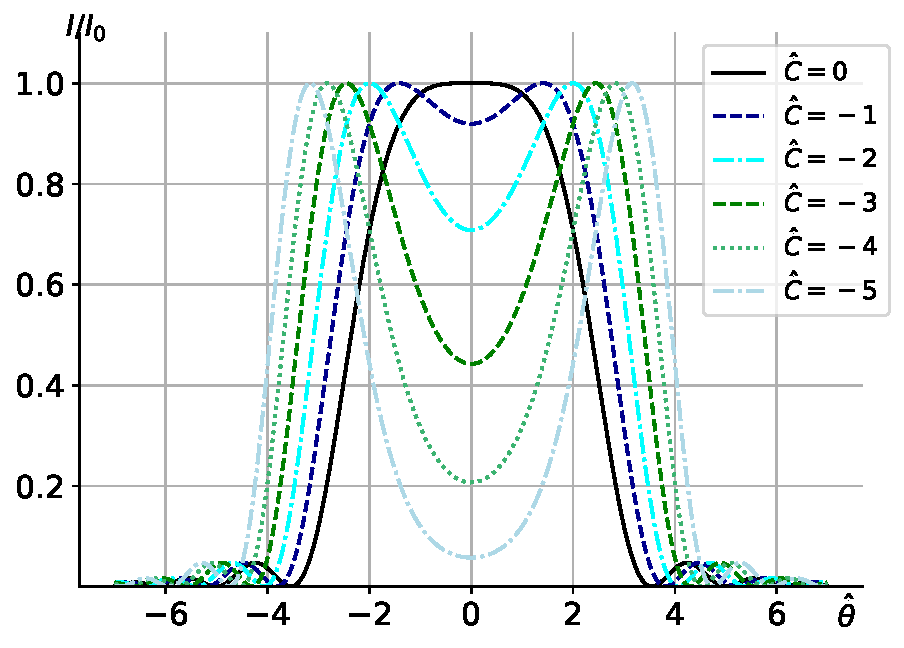
\includegraphics[width=\textwidth]{pic/angleC_neg.pdf}
		\caption{Угловое распределение поля при отрицательной сдвижке частоты}
		\label{fig:angle_dist_C_neg}
	\end{minipage}\hfill
	\begin{minipage}{0.49\textwidth}
		\centering
		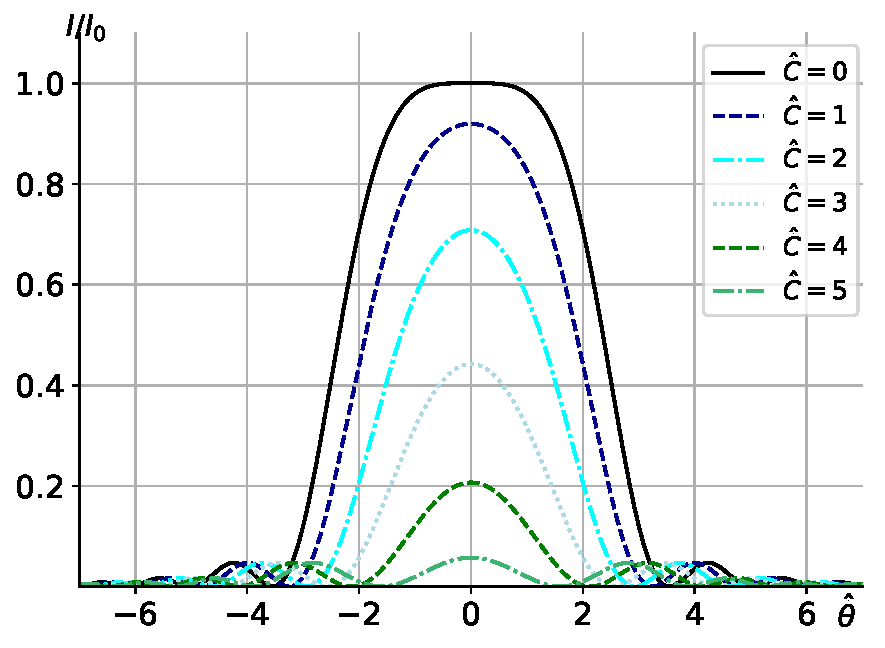
\includegraphics[width=\textwidth]{pic/angleC_pos.pdf}
		\caption{Угловое распределение поля при положительной сдвижке частоты}
		\label{fig:angle_dist_C_pos}
	\end{minipage}    
\end{figure}
На рис.~\ref{fig:angle_dist_C_neg} и рис.~\ref{fig:angle_dist_C_pos} изображены угловые распределения излучения. Их структуру можно понять из рисунка~\ref{fig:traj}. Конструктивная интерференция наблюдается на оси, где есть максимум интерференционной картины на резонансной частоте. Если произвести отрицательную сдвижку по частоте, то выполнение условия конструктивной интерференции: $n \lambda_{ph} = s_{ph} - \lambda_u \cos\theta$ будет наблюдаться при ненулевых углах наблюдения, и обратно, при положительной сдвижке частоты, интенсивность быстро падает, условие резонанса не может выполниться при меньших длинах волн на ненулевых углах, потому что в набег фазы на каждом периоде ондулятора, не укладывается целое число длин волн соответствующей гармоники излучения. Говорят, что электрон на каждом периоде ондулятора интерферирует сам с собой. Естественно, говорят о интерференции излучения, которое на оси обгоняет электрон на одну длину волны (или болеешее число волн, т.е. 1, 2, 3 и т.д.). На следующем периоде ондулятора, электрон снова излучает в фазе с излучённой на прошлом периоде волной. Важной характеристикой в приложениях является проинтегрированный по углам $\hat{\theta}$ спектр излучения, см. рис.~\ref{fig:spec_integrate_angle}. В некотором смысле, у спектра появляется широкий хвост. Форма спектра и единицы измерения для некоторой конкретной задачи должны обсуждаться отдельно.  
\begin{figure}[htbp]
	\centering
	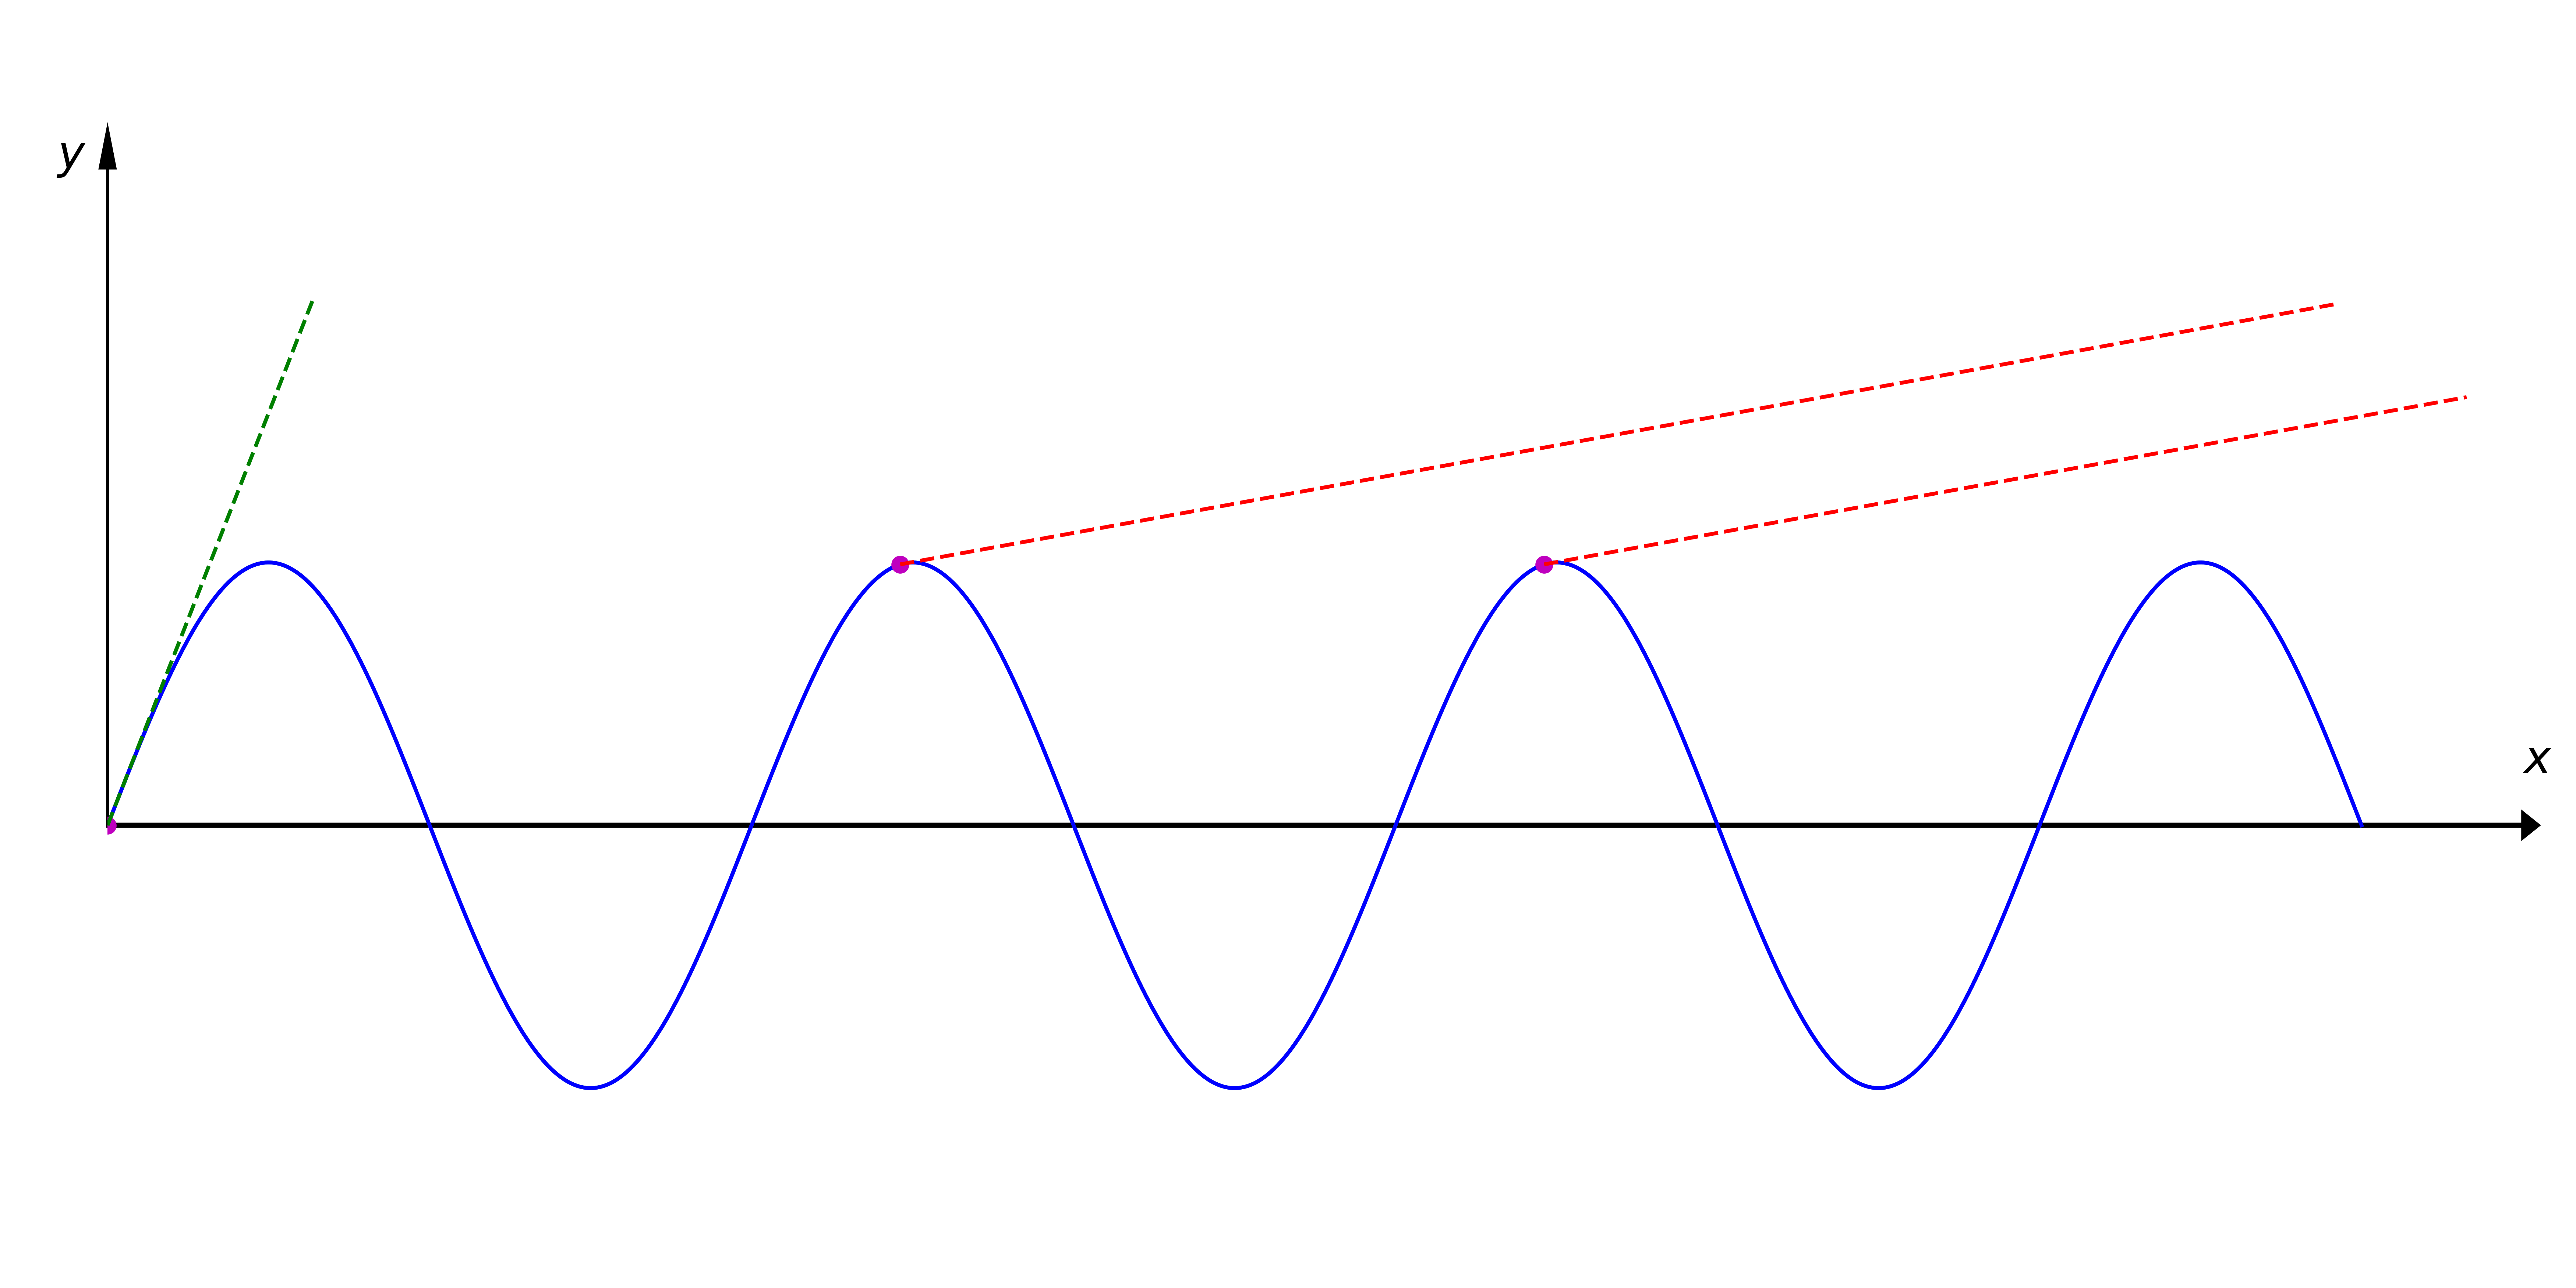
\includegraphics[width=.99\textwidth]{{pic/traj}.pdf}
	\caption{Ондулятор как интерференционное устройство} 
	\label{fig:traj}
\end{figure}

\begin{figure}[h!]
	\centering
	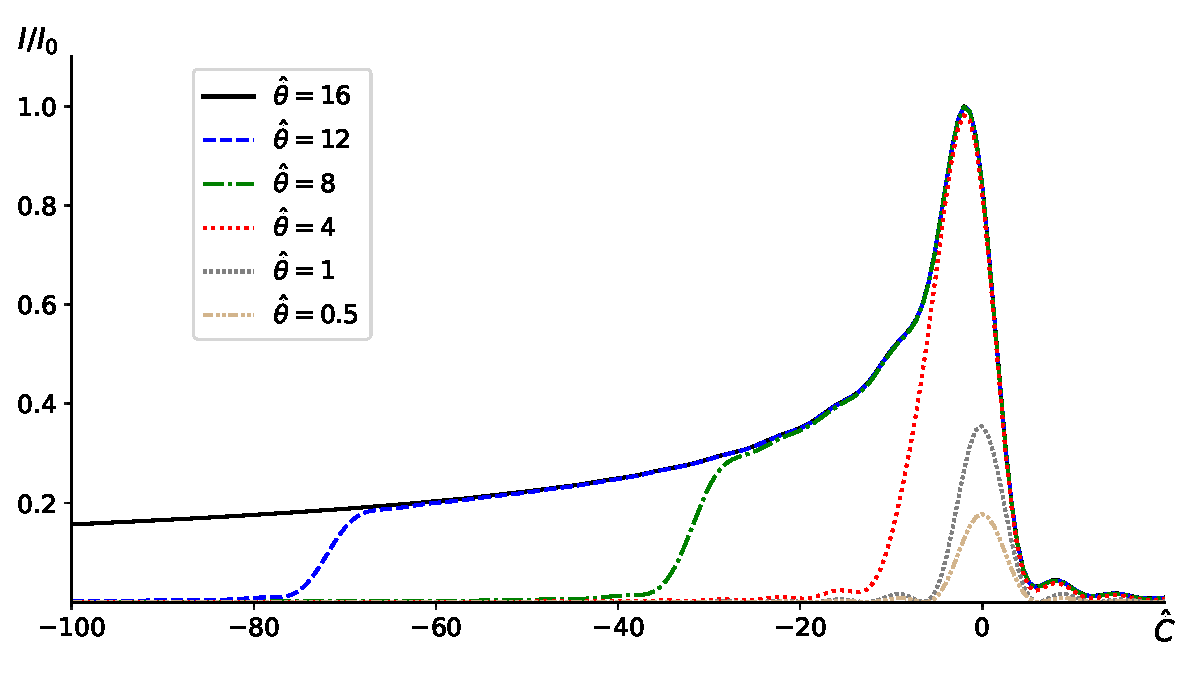
\includegraphics[width=.99\textwidth]{{pic/spec_integ_ang}.pdf}
	\caption{Проинтегрированный по углам спектр излучения. За $\hat{\theta}$ в легенде обозначены пределы интегрирования по углам} 
	\label{fig:spec_integrate_angle}
\end{figure}

\section{Излучение высших гармоник}
\subsection{Амплитудный спектр высших гармоник ондуляторного излучения в зависимости от параметра ондуляторности}
В этом разделе мы дадим описание свойств излучения высших гармоник. Начнём с объяснения амплитудного спектра ондуляторного излучения. Понимание данного вопроса необходимо в виду того, что выбор конкретных параметров ондулятора, обычно говорят о параметре ондуляторности $K$, чрезвычайно важен для приложений. Выбор этого параметра напрямую влияет на состав спектра излучения и его амплитудное распределение. Следуя выкладками~\ref{eq:field_dist_nonNorm}, где было введено обозначение $A_{JJ}$, и общей формуле для произвольной гармоники из \cite{wiedemann2015particle} можно написать:
\begin{equation}
	\label{eq:A_JJ}
	A_{JJ}(K) = \cfrac{n^2 K^2}{(1 + K^2/2)^2} \bigg[ J_{\frac{1}{2}(k-1)}\bigg(\cfrac{nK^2}{4 + 2K^2}\bigg) - J_{\frac{1}{2}(k+1)}\bigg(\cfrac{nK^2}{4 + 2K^2}\bigg)\bigg]^2,
\end{equation}
\begin{figure}[h]
	\centering 
	\begin{minipage}{0.99\textwidth}
		\centering
		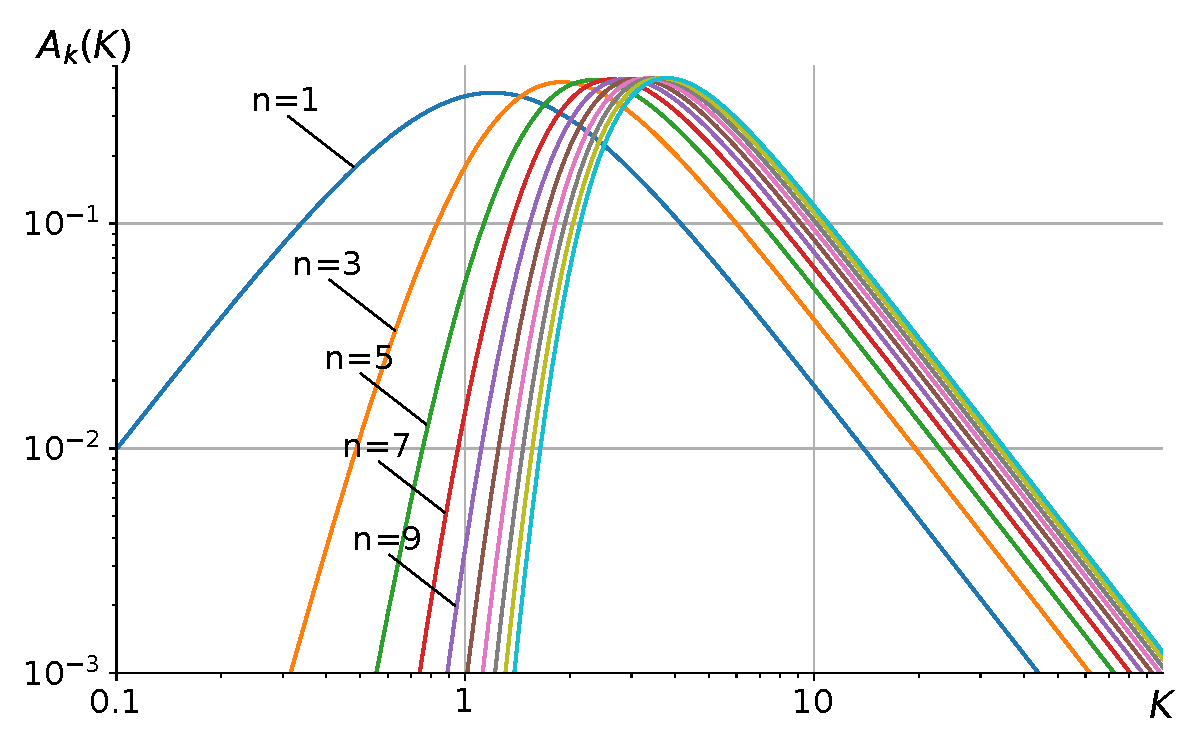
\includegraphics[width=.79\textwidth]{{pic/A_K}.pdf}
		\caption{Амплитудный спектр гармоник в зависимости от параметра ондуляторности $K$} 
		\label{fig:A_K}
	\end{minipage}
\end{figure}

Графическое представление этой формулы в зависимости от параметра $K$ показано на рис.~\ref{fig:A_K}. Спектр наглядно показывает зависимость амплитуд гармоник от параметра ондуляторности. На ондуляторах, где планируется работать на низших гармониках, преимущественно выбираются малые $K < 2$, если же стоят задачи, где используются более высокие гармоники, то параметр $K$ выбирают в районе $2 - 2,5$.

На рис.~\ref{fig:spec_und_1-1} и рис.~\ref{fig:spec_und_1-2} представлены примеры спектров ондуляторного излучения электронного пучка с бесконечно малым эмиттансом. Рисунки наглядно поясняют соображения изложенные выше по амплитудному составу ондуляторного спектра. Уже при при $K = 2,5$ максимум амплитуды приходиться на $7$-ую гармонику.
\begin{figure}[ht!]
	\begin{minipage}{0.49\textwidth}
		\centering
		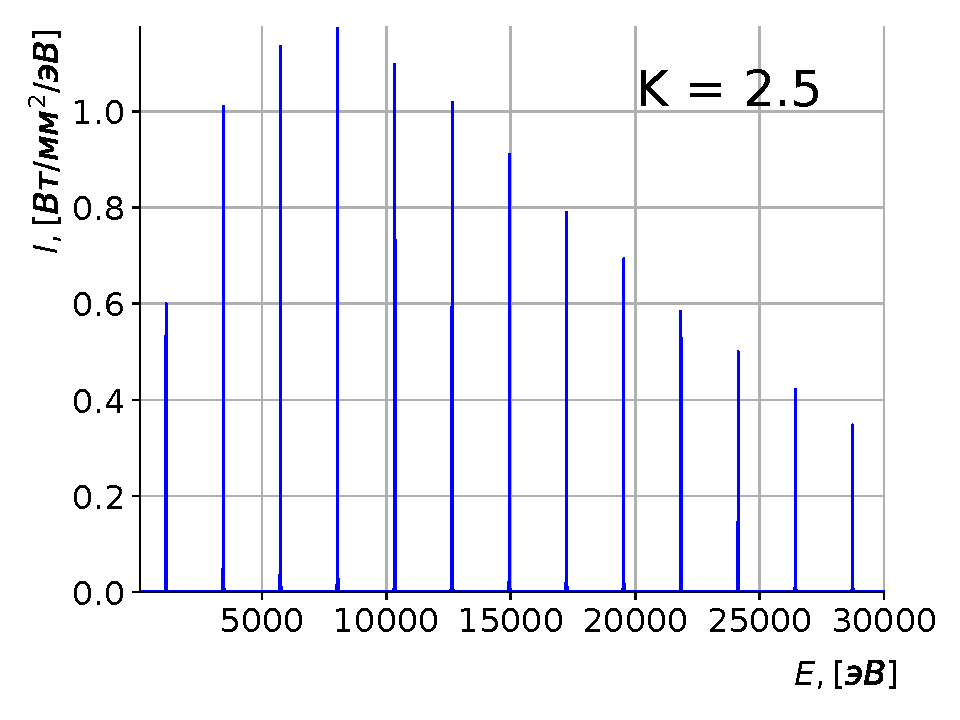
\includegraphics[width=\textwidth]{pic/spec_und_1-1.pdf}
		\caption{Спектр ондулятора с ондуляторностью $K = 2,5$}
		\label{fig:spec_und_1-1}
	\end{minipage}
	\begin{minipage}{0.49\textwidth}
		\centering
		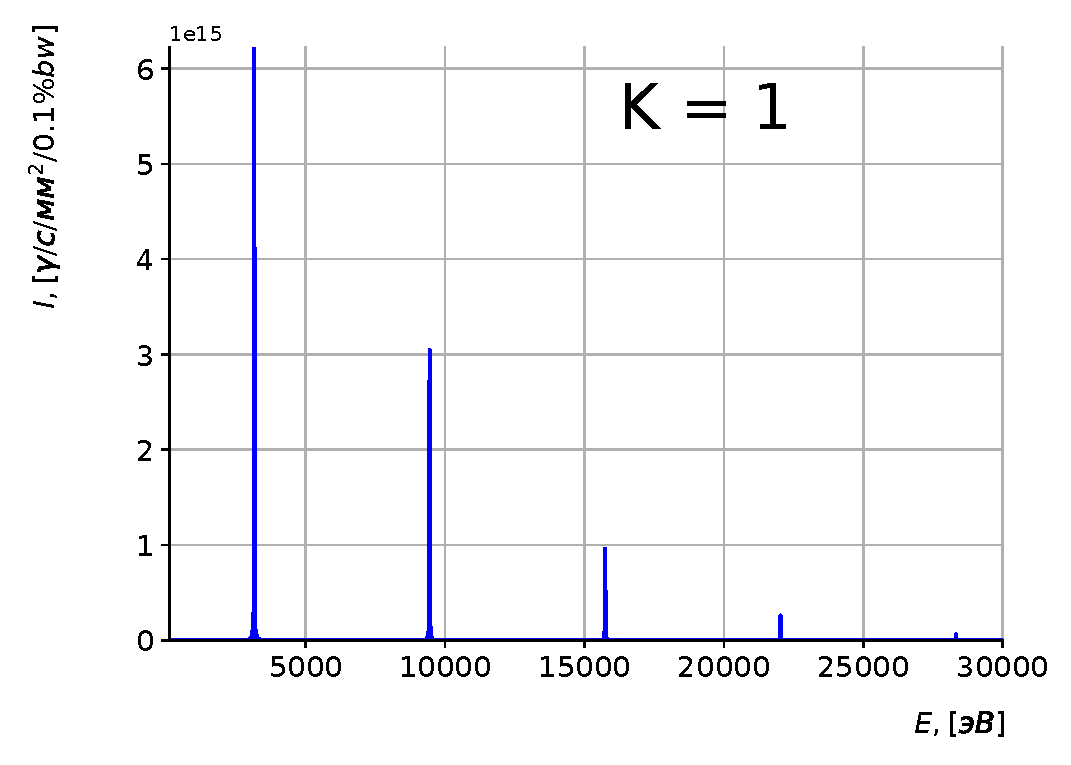
\includegraphics[width=\textwidth]{pic/spec_und_1-2.pdf}
		\caption{Спектр ондулятора с ондуляторностью $K = 1$}
		\label{fig:spec_und_1-2}
	\end{minipage}    
\end{figure}

\section{Заключение}









